\documentclass{article}


\usepackage{arxiv}

\usepackage[utf8]{inputenc} % allow utf-8 input
\usepackage[T1]{fontenc}    % use 8-bit T1 fonts
\usepackage{hyperref}       % hyperlinks
\usepackage{url}            % simple URL typesetting
\usepackage{geometry}
\geometry{margin=0.5in}
\usepackage{multirow}
\usepackage{float}
\usepackage{graphicx}
\usepackage{caption}
\usepackage{filecontents}
\usepackage{subcaption} % Add the subcaption package
\usepackage[title]{appendix}
\usepackage{fancyhdr}
\usepackage{array}
\usepackage{booktabs}       % professional-quality tables
\usepackage{amsfonts}       % blackboard math symbols
\usepackage{nicefrac}       % compact symbols for 1/2, etc.
\usepackage{microtype}      % microtypography
\usepackage{lipsum}
\usepackage{graphicx}
\pagestyle{fancy}
\graphicspath{ {./images/} }
\usepackage[compact]{titlesec}         % you need this package
\titlespacing{\subsection}{0pt}{5pt}{0pt} % this reduces space between (sub)sections to 0pt, for example


\title{COMP 551 Assignment 2 Report - Fall 2024}


\author{
 Hathaway Hao \\
  261071268\\
  %% examples of more authors
   \And
 Yifan Lin \\
  261078741\\
  \And
 Michael Yu \\
  261070826\\
  %% \AND
  %% Coauthor \\
  %% Affiliation \\
  %% Address \\
  %% \texttt{email} \\
  %% \And
  %% Coauthor \\
  %% Affiliation \\
  %% Address \\
  %% \texttt{email} \\
  %% \And
  %% Coauthor \\
  %% Affiliation \\
  %% Address \\
  %% \texttt{email} \\
}

\begin{document}
\maketitle
\begin{abstract}
\textit {Statistical learning is key to Machine Learning, so we evaluated linear regression and logistic classification on the Infrared Thermography and CDC Diabetes datasets. We implemented analytical least squares, gradient descent, and mini-batch SGD. Our experiments analyzed performance, feature importance, and the effects of training size, mini-batch size, and learning rates. Cross-validation was used to prevent overfitting, and we compared analytical and iterative approaches for linear regression. Key findings show the importance of learning rates, batch size, and computational trade-offs. This study marks our first application of machine learning and identifies areas for future research.}

\end{abstract}



\section{Task 1: Linear Regression with Non-Linear Basis Functions}
\subsection{Introduction}
The main objective of Task 1 is to explore the effectiveness of Gaussian basis functions in approximating non-linear relationships. We aim to demonstrate how increasing the complexity of a model by adding more basis functions affects its performance, highlighting the trade-off between underfitting and overfitting. Our approach starts with generating synthetic data from a non-linear function, and then attempting to approximate this function using a linear combination of Gaussian basis functions. We then can observe how model complexity by changing the number of basis functions, which influences the quality of fit and generalization performances.

\subsection{Methodology}

We began by generating a synthetic dataset that represents a non-linear relationship. The true function is defined as:
\[
y(x) = \sin(\sqrt{x}) + \cos(x) + \sin(x) + \epsilon
\]
Where $x$ is uniformly sampled from the range $[0, 20]$, and $\epsilon$ is Gaussian noise with mean 0 and variance 1.
\begin{figure}[H]
    \centering
    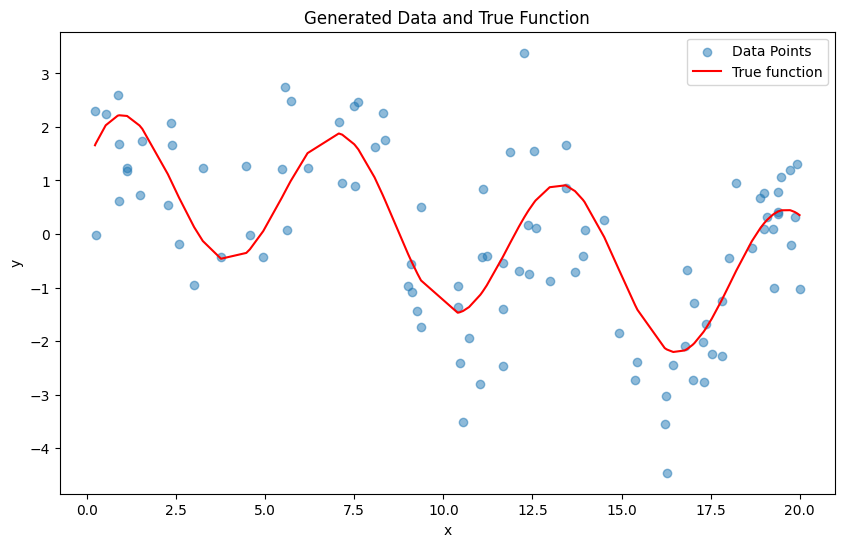
\includegraphics[width=0.5\linewidth]{figures/data.png}
    \caption{Smoothed Loss Function of Linear Regression with Mini-Batch Stochastic Gradient Descent with Learning Rate: 1e-1, 1e-2, 1e-3, 1e-4, 1e-5}
    \label{learning rate}
\end{figure}



\subsection{Data Processing}
Both datasets were preprocessed with a structured pipeline to ensure compatibility with the machine-learning models. The preprocessing steps are detailed below:
\begin{itemize}
    
    \item \textbf{Data Preparation and Exploration for both Datasets} \\
    Initially, data were loaded from the UCI repository. Basic data exploration was performed, which revealed the presence of some missing values in the dataset. For the \textit{Infrared Thermography Temperature} dataset, we conducted further exploration of each feature column, which led us to apply appropriate preprocessing techniques. Categorical variables such as 'Age', 'Gender', and 'Ethnicity' were \textbf{one-hot encoded} to convert them into numerical form. Boolean variables were also transformed into integers (0 or 1) to facilitate model training.
    \item \textbf{Handling Missing Values} \\
    After analyzing the dataset, we identified rows with missing values. These rows were removed to ensure the integrity of the data, leaving us with a clean dataset without null entries.
    \item \textbf{Feature-Target Exploration}  \\
    Since the target variable for the \textit{Infrared Thermography Temperature} dataset ('aveOralM') is continuous, we focused on exploring the relationship between the features and the target through visualizations such as scatter plots to understand how each feature impacts the target temperature.
    \item \textbf{Data Splitting and Normalization} \\
    Before training, both datasets were split into training and testing sets using an 80-20 split. After splitting, we applied standardization (scaling the data) to the feature sets using the \texttt{StandardScaler} to ensure that the features are on a similar scale. This helps the model converge faster during training. For the \textit{Infrared Thermography Temperature} dataset, the target variable 'aveOralM' was separated from the features after ensuring that all missing values were handled appropriately.
\end{itemize}



\section{Results}
\label{sec:results}

As stated in the introduction section, our study encompasses a series of experiments. To test our models, we conducted a series of experiments that are fundamental in machine learning research and practice. We evaluated performance metrics (MSE for regression, accuracy for classification) to establish baseline model effectiveness \ref{statistical learning}. We tested the impact of training data size to assess model scalability and data efficiency, as well as mini-batch size experiments, which helped optimize the takeaways between computational efficiency and convergence speed \ref{ref:lectures}. Cross-validation was employed to obtain robust performance estimates and avoid overfitting \ref{ref:validation}. Lastly, comparing analytical and iterative solutions provided insights into the strengths and limitations of different optimization approaches.

\subsection{Experiment 1: Report performance of linear regression for data1 and logistic regression for data2}

In this experiment, we evaluated the performance of the linear regression model using the Mean Squared Error (MSE), R-squared score, and Mean Absolute Error (MAE) for both the training and test sets.

\begin{table}[H]
    \centering
    \begin{minipage}{0.4\textwidth} % Adjust the width as needed
        \centering
        \resizebox{\textwidth}{!}{%
        \begin{tabular}{|c|c|c|c|}
            \hline
            \textbf{Set} & \textbf{MSE} & \textbf{R²} & \textbf{MAE} \\
            \hline
            Training & 0.0617 & 0.7756 & 0.1950 \\
            Test     & 0.0667 & 0.6646 & 0.2032 \\
            \hline
        \end{tabular}}
        \vspace{7pt}
        \caption{MSE, R², and MAE for Training and Test Sets of the Linear Regression Model}
        \label{table MSE linear}
    \end{minipage}
    \hfill
    \begin{minipage}{0.55\textwidth} % Adjust the width as needed
        \centering
        \resizebox{\textwidth}{!}{%
        \begin{tabular}{|c|c|c|c|c|}
            \hline
            \textbf{Set} & \textbf{Accuracy} & \textbf{Precision} & \textbf{Recall} & \textbf{F-1 score} \\
            \hline
            Training & 0.8627 & 0.5241 & 0.1683 & 0.2547 \\
            Test     & 0.8637 & 0.5332 & 0.1692 & 0.2569 \\
            \hline
        \end{tabular}}
        \vspace{7pt}
        \caption{Accuracy, Precision, Recall, and F-1 score for Training and Test Sets of the Logistic Regression Model}
        \label{table Accuracy Logistic}
    \end{minipage}
\end{table}


\noindent From the results shown in Table \ref{table MSE linear} and Table \ref{table Accuracy Logistic}, we can draw the following conclusions:

The Training MSE is 0.0617, while the Test MSE is 0.0667. The small difference between these values indicates that the model generalizes well, with minimal overfitting.
The R-squared values showing that the model explains 77.56\% of the variance in the training data and 66.46\% in the test data. Although the test set R-squared is slightly lower, this is expected and suggests a slight reduction in model performance on unseen data.
The MAE values for the training and test sets are also very close, shows that the average error in the model’s predictions is consistent across both sets.
Overall, the linear regression model demonstrates reasonable performance on both the training and test sets, with a slight decrease in accuracy on the test set, which suggests potential for further optimization or regularization.

The \textbf{Logistic Regression model} achieved a training accuracy of 0.8627 and test accuracy of 0.8637. Precision was moderate, at 0.5241 for training and 0.5332 for testing, while recall was low at around 0.17 for both sets, resulting in F1-scores of 0.2547 for training and 0.2569 for testing. Regularization did not improve performance, suggesting the need for more advanced techniques like handling class imbalance or feature engineering to boost recall and predictive performance.

\subsection{Experiment 2: Linear Regression vs. SGD Linear Regression}

In this experiment, we investigated the weights of the top 10 features in both traditional Linear Regression and Stochastic Gradient Descent (SGD) Linear Regression models. By examining feature weights, we gain insights into which variables most strongly influence the model's predictions, potentially uncovering non-obvious relationships in the data. Comparing top features from both approaches allows us to assess the consistency of feature importance across optimization methods, providing insights into the stability of our rankings. Additionally, this analysis can help detect potential biases in the dataset or model, prompting further investigation when unexpected features show large weights. The data evaluation is shown in Table \ref{linear features} and Table \ref{SGD linear features}:

\begin{table}[H]
    \centering
    \begin{minipage}{0.45\textwidth} % Adjust the width as needed
        \centering
        \resizebox{\textwidth}{!}{%
        \begin{tabular}{|c|c|c|}
            \hline
            \textbf{Feature} & \textbf{Weight} & \textbf{Absolute Weight} \\
            \hline
            canthi4Max1   & 0.357622  & 0.357622 \\
            canthiMax1    & -0.352782 & 0.352782 \\
            T\_Max1       & 0.301124  & 0.301124 \\
            T\_LC1        & 0.300552  & 0.300552 \\
            T\_RC\_Max1   & 0.230246  & 0.230246 \\
            T\_OR1        & 0.212044  & 0.212044 \\
            Max1R13\_1    & -0.209065 & 0.209065 \\
            T\_RC1        & -0.159100 & 0.159100 \\
            T\_OR\_Max1   & -0.157372 & 0.157372 \\
            T\_RC\_Dry1   & 0.143177  & 0.143177 \\
            \hline
        \end{tabular}}
        \vspace{7pt}
        \caption{Top 10 Features by Absolute Weights in Linear Regression}
        \label{linear features}
        
    \end{minipage}
    \hfill
    \begin{minipage}{0.45\textwidth} % Adjust the width as needed
        \centering
        \resizebox{\textwidth}{!}{%
        \begin{tabular}{|c|c|c|}
            \hline
            \textbf{Feature} & \textbf{Weight} & \textbf{Absolute Weight} \\
            \hline
            T\_FHLC1      & -0.199022 & 0.199022 \\
            T\_RC\_Wet1   & 0.195939  & 0.195939 \\
            RCC1          & -0.188584 & 0.188584 \\
            Max1L13\_1    & -0.163420 & 0.163420 \\
            T\_Max1       & 0.142402  & 0.142402 \\
            aveAllL13\_1  & 0.108773  & 0.108773 \\
            T\_FHBC1      & 0.106191  & 0.106191 \\
            T\_atm        & -0.099799 & 0.099799 \\
            T\_RC\_Dry1   & 0.085703  & 0.085703 \\
            canthiMax1    & 0.078252  & 0.078252 \\
            \hline
        \end{tabular}}
        \vspace{7pt}
        \caption{Top 10 Features by Absolute Weights in SGD Linear Regression}
        \label{SGD linear features}
    \end{minipage}
\end{table}


\subsection{Experiment 3: Influence of Training Data Size on Linear Regression Loss}
Experiment 3 investigates the influence of training data size on model performance for both linear and logistic regression. This analysis is crucial for understanding how much data is needed for effective model training and how model performance scales with increased data availability. By varying the proportion of data used for training from 20\% to 80\%, we can observe the learning curve of each model and identify potential overfitting or underfitting scenarios.
\noindent From the results shown in Table \ref{linear train size} \ref{logistic train size} and Figure \ref{linear train size figure}\ref{logistic train size figure}, we can draw the following key conclusion:


\begin{figure}[H]
    \centering
    \begin{minipage}{0.45\textwidth}  % Adjust the width as needed
        \centering
        \includegraphics[width=0.8\textwidth]{figures/experiment3_linear.png}  % Include the image
        \caption{Impact of Training Data Size on Linear Regression Model Performance}
        \label{linear train size figure}
    \end{minipage}
    \hfill
    \begin{minipage}{0.45\textwidth}  % Adjust the width as needed
        \centering
        \includegraphics[width=0.8\textwidth]{figures/experiment3_logistic.png}  % Include the image

        \caption{Impact of Training Data Size on Logistic Regression Model Performance}
        \label{logistic train size figure}
    \end{minipage}
\end{figure}

As the \textbf{training data size increases}, the \textbf{loss decreases}. More specifically:

For the Linear Regression model, performance is highly volatile at smaller training sizes (20-50\%). Then A significant improvement occurs at 60\% training size, with loss decreasing to 7.1. Finally, The model achieves its best performance at 70-80\% training size, with losses of 0.065 and 0.0635 respectively. For the Logistic Regression model, performance is remarkably consistent across all training sizes, with losses ranging narrowly from 0.3189 to 0.3213. There's a slight trend of decreasing loss as training size increases, but the difference is minimal.

\subsection{Experiment 4: Mini-Batch Size Impact on Convergence and Performance}

\begin{figure}[h]
    \centering
    \begin{minipage}{0.49\textwidth}
        \centering
        \includegraphics[width=\linewidth]{figures/minibatch.png}
    \end{minipage}
    \hfill
    \begin{minipage}{0.49\textwidth}
        \centering
        \includegraphics[width=\linewidth]{figures/e4_log.png}
    \end{minipage}
    \caption{Influence of Mini-batch Size on our Linear Regression Loss (smoothed) with Mini-Batch Stochastic Gradient Descent}
    \label{minibatch}
\end{figure}

In Figure \ref{minibatch}, these line graphs show that larger mini-batch sizes generally lead to better performance in SGD linear regression. As batch size increases from 8 to full batch, we see more stable convergence and lower final loss values. Compared to a fully batched approach, the larger mini-batches seem to approach similar performance levels. While larger batches converge more slowly initially, they ultimately provide better stability and final results. Among the tested configurations, full batch size 814 works best, offering optimal performance and stability.


\subsection{Experiment 5: Try different learning rates}
In this experiment, we investigated the impact of different learning rates on the performance of a Stochastic Gradient Descent (SGD) Linear Regression model. We tested five different learning rates: 1e-1, 1e-2, 1e-3, 1e-4, and 1e-5, over 1500 iterations with a batch size of 32. The experiment data visualization is shown below \ref{learning rate}:
\begin{figure}[H]
    \centering
    \includegraphics[width=0.8\linewidth]{figures/experiment5.png}
    \caption{Smoothed Loss Function of Linear Regression with Mini-Batch Stochastic Gradient Descent with Learning Rate: 1e-1, 1e-2, 1e-3, 1e-4, 1e-5}
    \label{learning rate}
\end{figure}

\begin{figure}[H]
    \centering
    \includegraphics[width=0.8\linewidth]{figures/experiment5_logistic.png}
    \caption{Smoothed Loss Function of Logistic Regression with Learning Rate: 1e-1, 1e-2, 1e-3, 1e-4, 1e-5}
    \label{learning rate}
\end{figure}

For this problem and dataset, a learning rate of 1e-2 appears to be optimal among the tested values. It provides the best balance between convergence speed and stability. Learning rates that are too high cause (1e-1) the model to diverge, while rates that are too low (1e-4 \& 1e-5) cause the model to converge too slowly.

In this experiment, we evaluated the effect of different learning rates on the loss in a logistic regression model. The learning rate significantly impacts how fast or slow the model converges, as seen in the results across various rates. Overall, the learning rate of 0.1 was optimal for this experiment, leading to the lowest loss and fastest convergence, while smaller learning rates hindered the model’s performance and slowed its learning.

\subsection{Experiment 6: Perform cross-validation using different learning rates}

In this experiment, we evaluated the performance of both our linear regression and logistic regression models using optimal parameters. The performance metrics for the linear regression model, as shown in Table \ref{Cross-Validation: Linear Regression}, include the Mean Squared Error (MSE) for both training and test sets. The model demonstrates an MSE of 0.264627 on the training set and 0.387184 on the test set, indicating that the model generalizes well without significant overfitting.

\begin{table}[H]
    \begin{subtable}{0.5\textwidth} % First table for MSE
        \centering
        \vspace{7pt}
        \renewcommand{\arraystretch}{1.5}
        \begin{tabular}{|c|c|}
            \hline
            Set  & MSE \\
            \hline
            Training Set & 0.264627 \\
            Test Set & 0.387184 \\
            \hline
    
        \end{tabular}
        \caption{\textbf{Table 4} 5-Fold Cross-Validation in linear}
        \label{Cross-Validation: Linear Regression}
    \end{subtable}%
    \begin{subtable}{0.5\textwidth} % Second table for Accuracy, Precision, Recall, F1-score
        \label{Cross-Validation: Logistic Regression}
        \centering
        \vspace{7pt}
        \renewcommand{\arraystretch}{1.5}
        \begin{tabular}{|c|c|c|c|c|}
            \hline
            \textbf{Set}    & \textbf{Accuracy} & \textbf{Precision} & \textbf{Recall} & \textbf{F1-score} \\
            \hline
            Training        & 0.862781          & 0.862067           & 0.864027        & 0.863005          \\
            \hline
            Test            & 0.863076          & 0.863464           & 0.863181        & 0.863128          \\
            \hline
        \end{tabular}
    \caption{\textbf{Table 5} 5-Fold Cross-Validation in logistic}
    \label{Cross-Validation: Logistic Regression}
    \end{subtable}
    
\end{table}
Additionally, Table \ref{Cross-Validation: Logistic Regression} presents the accuracy, precision, recall, and F1-score for the logistic regression model on both the training and test sets. The model achieves an accuracy of 0.862781 on the training set and 0.863076 on the test set, with similar high values for precision, recall, and F1-score. These results suggest that the logistic regression model performs consistently across both datasets, confirming its robustness and generalization ability.


\subsection{Experiment 7: Compare analytical solution with mini-batch SGD}
Here in figure \ref{comparison}, the analytical solution provides a constant loss value, serving as a baseline for optimal performance. In contrast, the SGD approach shows an evolution of performance over iterations. Initially, the SGD loss is significantly higher than the analytical solution, reflecting the random initialization of weights. As the number of iterations increases, the SGD loss rapidly decreases and then begins to oscillate around the analytical solution's loss value. This oscillation is characteristic of SGD, resulting from the stochastic mini-batch sampling and the fixed learning rate.

\begin{figure}[H]
        \centering
        \includegraphics[scale=0.3]{figures/Comparison.png}

    \caption{The comparison between linear regression and Mini-batch SGD}
    \label{comparison}
\end{figure}




\section{Discussion and Conclusion}

Here are our takeaways from all the experiments we have made:

\begin{itemize}
    \item \textbf{Experiment 1} \\
    The linear regression model generalized well, while logistic regression had high accuracy but struggled with precision-recall balance. Regularization was ineffective, and further improvements should focus on class imbalance and feature engineering. Both models performed adequately but need refinement. Limitation: Performance may degrade on larger datasets due to computational constraints.

  \item \textbf{Experiment 2}  \\
    We compared feature importance between Linear and SGD Linear Regression. The top features were consistently ranked, though some biases in weights suggest further investigation is needed.Limitation: Results may vary with larger datasets or different SGD hyperparameters.

  \item \textbf{Experiment 3} \\
    We examined how training size affects performance. Linear regression was volatile with small data but improved with more. Logistic regression remained stable across all sizes, suggesting it handles small datasets better. Limitation: Larger datasets may reveal different behaviors or performance issues not observed with smaller samples.

  \item \textbf{Experiment 4} \\
    Using a full batch size of 814 provided the best balance between stability and performance, resulting in the lowest loss. Smaller batches had more volatile convergence, while larger batches converged more slowly but more consistently. The limitation is that only a few batch sizes were tested; further tuning and testing with different datasets could offer additional insights.

  \item \textbf{Experiment 5} \\
  A learning rate of 0.1 provided the best balance between speed and stability in this experiment, leading to the lowest loss and fastest convergence. Higher rates caused divergence, while lower rates led to slow convergence. The limitation is that we only tested a few rates; further tuning and additional iterations could provide deeper insights.

  \item \textbf{Experiment 6}  \\
    We assessed the performance of linear and logistic regression with optimal parameters. Linear regression generalized well, showing minimal overfitting, while both models benefited from improved stability and reduced errors. Logistic regression demonstrated consistent accuracy across datasets, highlighting the value of parameter optimization. Limitation: Further tuning may be needed for larger or more complex datasets.


  \item \textbf{Experiment 7} \\
    We compared analytical and SGD solutions for linear regression. SGD initially showed higher loss but converged towards the analytical solution over iterations. Limitation: The number of iterations was preset and longer runs might show different long-term behavior.

\end{itemize}

Future investigations could involve delving into deep neural networks to leverage their capability to capture complex patterns and perform comparisons with our current models. Additionally, probing into parameter tuning for these deep learning models, including factors such as learning rate, training data size, and mini-batch size, holds promise for enhancing their robustness on the datasets.



\section{Statement of Contributions}

All members contributed equally to this project. We each completed the lab independently and then combined our individual work and code to produce the final report.

\newpage
\bibliographystyle{unsrt}  
%\bibliography{references}  %%% Remove comment to use the external .bib file (using bibtex).
%%% and comment out the ``thebibliography'' section.

%%% Comment out this section when you \bibliography{references} is enabled.
\begin{thebibliography}{1}

\bibitem{Infrared Thermography Temperature} Infrared Thermography Temperature
Wang et al., 2021
https://api.semanticscholar.org/CorpusID:245585208
\label{ref:dataset1}

\bibitem{CDC Diabetes Health Indicators} CDC Diabetes Health Indicators. 2021. https://archive.ics.uci.edu/dataset/891/cdc+diabetes+health+indicators \label{ref:dataset2}

\bibitem{statistical learning} Hastie, Trevor, et al. The elements of statistical learning: data mining, inference, and prediction. Vol. 2. New York: springer, 2009. \label{statistical learning}

\bibitem{Lecture notes} Prémont-Schwarz, I. (2023). Gradient Descent. COMP 551, McGill University.\label{ref:lectures}

\bibitem{validation} James, Gareth. "An introduction to statistical learning." (2013) \label{ref:validation}

\end{thebibliography}

\begin{appendices}

\section{Default Model Parameters} \label{app:default-parameters}

\begin{table}[H]
    \centering
    \vspace{7pt} % Adjust the value as needed to control the amount of space
    \renewcommand{\arraystretch}{1.5}
    \begin{tabular}{|c|c|c|c|c|c|}
        \hline
        Model  & Max iteration & Batch Size & Learning Rate & Epsilon & Regularization Term \\
        \hline
        Linear Regression with SGD & 1500 & 16 & 1e-2 & 1e-5 & 0 \\
        Logistic Regression & 2000 & 16 & 1e-3 & 1e-7 & 0.1 \\
        \hline
    \end{tabular}
\end{table}

\section{Experiment 3}

\subsection{Training Loss History of Linear Regression with data size} \label{app:loss-history-sgd}

\begin{table}[h]
    \centering
    \begin{minipage}{0.45\textwidth}  % Adjust the width as needed
        \centering
        \begin{tabular}{|c|c|}
            \hline
            \textbf{Training Size (Proportion)} & \textbf{MSE Loss} \\
            \hline
            0.2  & 233.8436 \\
            0.3  & 100.6199 \\
            0.4  & 162.3182 \\
            0.5  & 11.3937  \\
            0.6  & 7.1098   \\
            0.7  & 0.0650   \\
            0.8  & 0.0635   \\
            \hline
        \end{tabular}
        \vspace{7pt}
        \caption{Linear in Different Training Set Sizes}
        \label{linear train size}
    \end{minipage}
    \hfill
    \begin{minipage}{0.45\textwidth}  % Adjust the width as needed
        \centering
        \begin{tabular}{|c|c|}
            \hline
            \textbf{Training Size (Proportion)} & \textbf{MSE Loss} \\
            \hline
            0.2  & 0.3201 \\
            0.3  & 0.3198 \\
            0.4  & 0.3195 \\
            0.5  & 0.3213  \\
            0.6  & 0.3191   \\
            0.7  & 0.3189   \\
            0.8  & 0.3198   \\
            \hline
        \end{tabular}
        \vspace{7pt}
        \caption{Logistic in Different Training Set Sizes}
        \label{logistic train size}
    \end{minipage}
\end{table}

\subsection{Final Loss, Mean Loss and Min Loss in Linear Regression model with different mini-batch SGD} \label{app:loss-history-sgd-log}
\begin{table}[h!]
    \centering
    \begin{tabular}{|c|c|c|c|}
        \hline
        \textbf{Batch Size} & \textbf{Final Loss} & \textbf{Mean Loss} & \textbf{Min Loss} \\
        \hline
        8   & 55391.013203 & 28565.609963 & 52.265444  \\
        16  & 2085.653474  & 149.216125   & 3.461185   \\
        32  & 0.101154     & 67.321424    & 0.086003   \\
        64  & 0.083188     & 65.046168    & 0.080201   \\
        128 & 0.068877     & 64.398326    & 0.068812   \\
        814 & 0.068739     & 63.514423    & 0.068739   \\
        \hline
    \end{tabular}
    \vspace{7pt}
    \caption{Summary of Mini-batch Size Influence on SGD Linear Regression Loss}
    \label{tab:sgd_loss}
\end{table}


\end{appendices}

\end{document}

